\chapter{Yet another tool: XCorex }\label{ch:3}

\epigraph{Programming today is a race between software engineers striving to
build bigger and better idiot-proof programs, and the Universe trying to produce
bigger and better idiots. So far, the Universe is winning.}{Rich Cook}

	For the problems presented in chapter \ref{ch:2.2} I have implemented a tool
that defines a meta-metamodel as described in chapter \ref{ch:2.1.1} which will
allow you to describe the metamodel for the tool you want to implement and it will generate 
a model based on the data you provided. In order to evaluate the application I
have also reimplemented a front-end tool called InsiderView \cite{tools:iPlasma}
which allows you to integrate different metrics based on the meta-metamodel from 
CodePro.
	During the implementation phase there were a number of different ideas
that were proposed and/or implemented in order to fully understand the
limitations of annotation processing and code generation in java and also to
provide the most general solution which can be used by as many users as
possible.

\section{XCorex}

\subsection{Solution Overview}
	 
\begin{figure}
\centering
\scalebox{0.5}{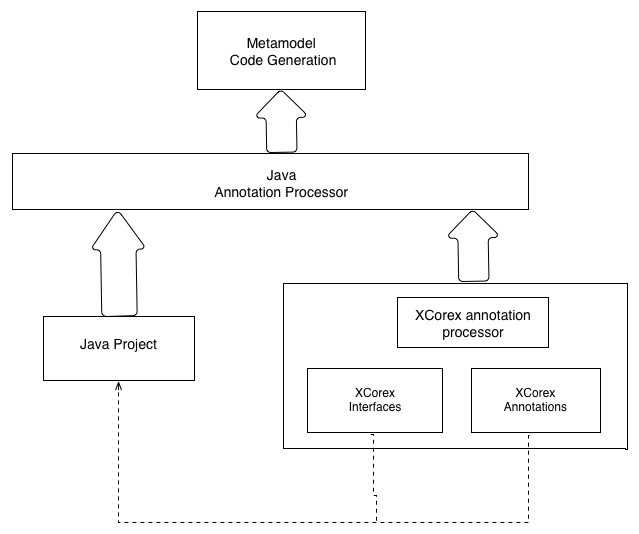
\includegraphics{../img/solution/XCorexSystem.png}}
\caption{XCorex System overview}
\label{fig:XCorexSystem}
\end{figure}

	Figure \ref{fig:XCorexSystem} represent the  general system architecture. 
As it can be seen there are three main components that describe the XCorex
system:
	\begin{itemize}
	  \item Annotation Component
	  \item Interface  Component
	  \item Annotation Processor
	\end{itemize}
	The XCore annotation component represent the implementation of the
meta-metamodel as presented in chapter \ref{ch:2.1.1} and provides the necessary
metadata to describe the metamodel which is implemented by the client. 
	The XCorex interface component helps the client in describing the necessary
elements for the model of the application and also enforces a type safe environment.
	The above two components describe the semantics of our system which is enforced 
by the annotation processor. The processor is, if you will, the brain of system
which analysis the metadata provided by client with the help of the two
components and generates the appropriate model. 

\subsection{Implementation Details}

\subsubsection{Annotation Component}

	The annotations we have defined combined with the interfaces, which will be
presented in the section below form the meta-metamodel of our program as
describe in section \ref{ch:2.1.1}.
	As you can see in the code sections below the annotations are only allowed to
annotate java types, to be more specific only classes, and help us distinguish between
group builders, which describe any type of relation between a series of elements of the same type, and property
computers which represent a general description of a metric. 

		\small
	\begin{lstlisting}[language=Java,numbers=left]
@Target(ElementType.TYPE)
public @interface GroupBuilder {}	
	\end{lstlisting}
	\normalsize{} \label{codeSection:GroupBuild}
	
		\small
	\begin{lstlisting}[language=Java,numbers=left]
@Target(ElementType.TYPE)
public @interface PropertyComputer {}
	\end{lstlisting}
	\normalsize{} \label{codeSection:PropertyComputer} 

\subsubsection{Interface Component}

	Both annotations presented above force the annotated type to implement a
specific interface which assures us type safety through generics. For the
GroupBuilder annotation we have the IGroupBuilder interface and for the
PropertyComputer annotation we have the IPropertyComputer interface, both
definitions can be seen below.

	\small
	\begin{lstlisting}[language=Java,numbers=left]
public interface IGroupBuilder <ElementType extends XEntity, 
                 Entity extends XEntity> {
	Group<ElementType> buildGroup(Entity entity);
}
	\end{lstlisting}
	\normalsize{} \label{codeSection:IGroupBuilder}
	
	For the GroupBuilder the ElementType represents the type for the aggregated
elements and the entity represent the aggregator type. For example if we want to
define the group of all methods for a class we would have something very
similar to:
	\small
\begin{lstlisting}[language=Java,numbers=left]
@GroupBuilder
public class ListOfMethods implements IGroupBuilder<XMethod, XClass> {
	@Override
	public Group<XMethod> buildGroup (XClass entity) {}
}
\end{lstlisting}
	\normalsize{} 
	
	\small
	\begin{lstlisting}[language=Java,numbers=left]
public interface IPropertyComputer <ReturnType, Entity extends XEntity> {
	ReturnType compute(Entity entity);
}	
	\end{lstlisting}
	\normalsize{} \label{codeSection:IPropertyComputer}
	
	The ReturnType can be any type which makes sens for the current metric
to return (Double, Integer, String, Pair<>, \ldots{} etc). 
	The XEntity represents a markup interface which define the elements of our
metamodel which we will be generating when the compilation process starts and
the annotation processor is invoked. The Entity type which is present in both 
interfaces must not exists before, because it will be generated.
		
\subsubsection{Annotation Processor}
	
	All of the elements presented above, annotations and interfaces, are defined 
by using the java syntax and thus we are confident that they will be used
correctly from that point of view, but they also have semantics attached which
cannot be enforced by syntax alone. In order to enforce the appropriate
semantics we have defined an annotation processor which will parse every
relevant project files, java files which contain elements annotated with the
elements presented in the sections above, it will analyze every elements and, if
needed, will generate the appropriate  errors or warnings.
	The process of discovering which elements are annotated and with what kind of
annotations is the responsibility of the compiler. Once our requested
annotations are identified the compiler will invoke the processor by calling
the \code{process(Set<? extends TypeElement> annotations,RoundEnvironment roundEnv)}
method with the annotations it identified and are relevant for us, and the
corresponding java elements that are attached to them. 
	Each element is processed, first starting with the PropertyComputers and
continuing with the GroupBuilders, and the following rules are enforced:
	
	\begin{itemize}
	  \item All elements that are annotated must be classes
	  \item All annotated classes must have a default constructor.
	  \item All elements annotated with @PorpertyComputer must implement
 IPropertyComputer
 	  \item All elements annotated with @GroupBuilder must implement
 IGroupBuilder
 	  \item  All classes cannot be present in the default package
 	  \item  The @PropertyComputer and @GroupBuilder annotations are mutually
exclusive
	  \item  No wildcard types are allowed to be specified for the entity type
 parameter.
	\end{itemize}
	When an invalid element is encounter an error similar to the one in figure
\ref{fig:xCorexError} is presented.
	For the rest of the elements, which are valid, the entity type defined in the
interface as a type parameter is extracted by using the mirror api provided by
the compiler and the appropriate code. For each unique entity type found, an
interface is generated which implements the XEntity markup interface and which
contains a method for every PropertyComputer that uses this type and a method
for every GroupBuilder which uses this entity for generating the elements of the
group. Also if any comments are associated with the PropertyComputers or
GroupBuilders they are preserved in the generated code. Figure
\ref{fig:xCorexCodeExample} and \ref{fig:xCorexRunExample} show an example on
how the code must be written and what is generated.

\begin{figure}
\centering
\scalebox{0.5}{\includegraphics{}}
\label{fig:xCorexCodeExample}
\end{figure}

\begin{figure}
\centering
\scalebox{0.5}{\includegraphics{}}
\label{fig:xCorexRunExample}
\end{figure}
	
	Each interface generated in the previous step is implemented by defining the
appropriate class in an impl package. The class will implement every method
defined in the interface by simply instantiating and object of the appropriate
PropertyComputer or GroupBuilder and call the compute method by passing a
reference to \code{this}. Also, there is one addition method that is implemented 
by each entity and this is the \code{getUnderlyingObject()} method which returns
the equivalent object from the framework we are using. For example if we are
using Eclipse JDT framework an equivalent for a XClass entity would be IType.
By default the method returns Object, but if the user specifies the type as
shown in figure \ref{fig:xCorexTypeDialogBox} the method will return the
specified type as can be seen in figure \ref{fig:xCorexUnderlyingObject}

\begin{figure}
\centering
\scalebox{0.5}{\includegraphics{}}
\label{fig:xCorexTypeDialogBox}
\end{figure}

	The implementation classes are not publicly available.
In order to be able to instantiate an element a FacetoryMethod class is
generated which also has cache support to increase speed and avoid useless
object instantiation.
	
	
\begin{figure}
\centering
\scalebox{0.5}{\includegraphics{}}
\label{fig:xCorexUnderlyingObject}
\end{figure}
	
\begin{figure}
\centering
\scalebox{0.4}{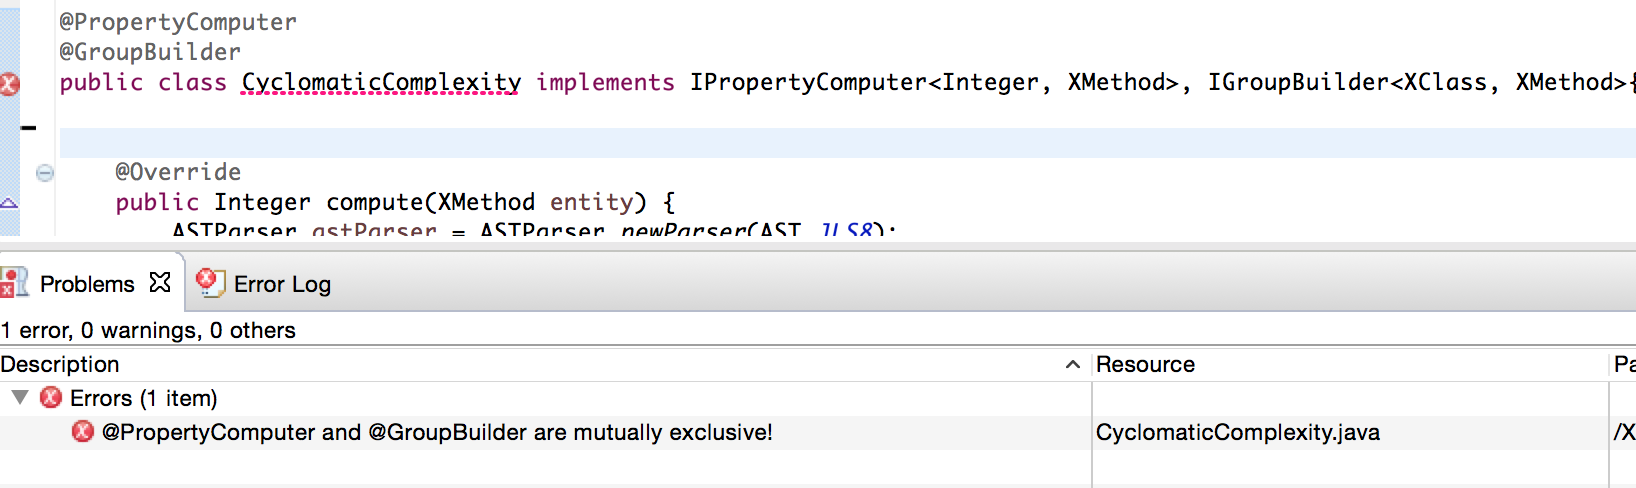
\includegraphics{../img/solution/xCorexError.png}}
\label{fig:xCorexError}
\end{figure}

\section {XCorexView}

\subsection {Overview}
	XCorexView is a tool based on XCorex which implements a series of  software
	metrics

\subsection {What has changed}

	